
\chapter{Multidimensional Visual Analysis (MVA)}

\label{chap:MVA}

Multidimensional Visual Analysis (MVA) refers to methods and techniques to
analyze and understand complex datasets using visual representations.
These approaches typically involve the use of specialized software or
tools that allow analysts to create and manipulate graphical
representations of the data in order to uncover patterns, trends, and
relationships. In this section, some popular MVA approaches are reviewed
\parencites{cao2011mva}[Chapter~2]{dzemyda2012mva}.



\section{Scatter Plots}

A scatter plot is a type of graph that is used to display the
relationship between two numerical variables, to identify any
potential trends or patterns in the data, and to identify outliers. It
uses dots or markers to represent the values of the two variables, and
position of each dot on the graph indicates the value of the two
variables in a single observation.

To create a scatter plot, the values of one variable are plotted on the
x-axis (horizontal axis) and the values of the other variable are plotted
on the y-axis (vertical axis). The resulting graph will show a set of
dots, with each dot representing a single observation. If there is a
positive relationship between the two variables, the dots will tend to
form a diagonal line that slopes upwards from left to right. If there is a
negative relationship, the dots will tend to form a diagonal line that
slopes downwards from left to right. If there is no relationship between
the two variables, the dots will be scattered randomly across the graph.
Figure~\ref{fig:ScatterplotDiagram} shows an example of a scatter plot
displaying data point on x-axis and on y-axis

\begin{figure}[tp]
\centering
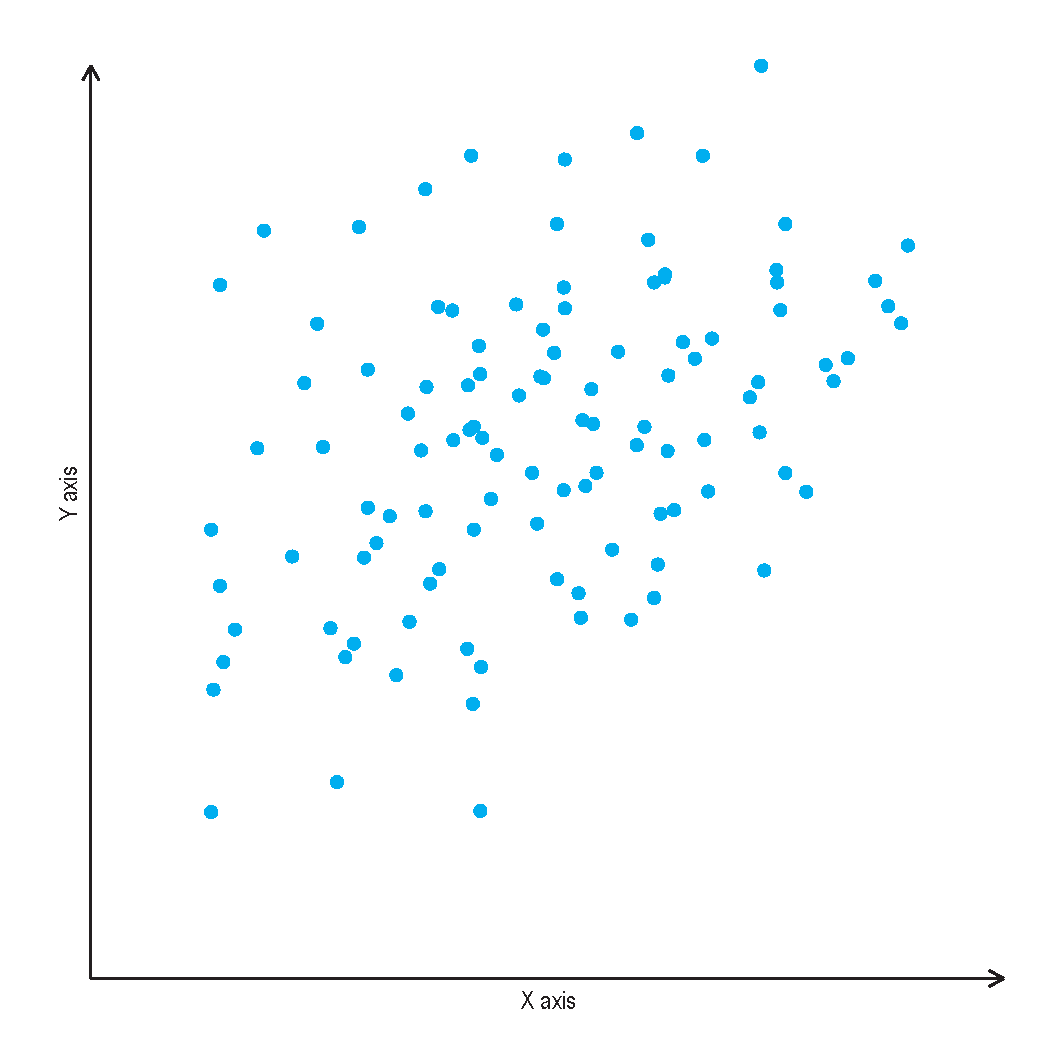
\includegraphics[frame,keepaspectratio,width=\linewidth,height=\halfh]
{diagrams/scatterplot.pdf}

\caption[Scatterplot]
{
A scatterplot displaying data points on x-axis and on y-axis.
\imgcredit{Drawn by Ožbej Golob using Adobe Illustrator.}
}
\label{fig:ScatterplotDiagram}
\end{figure}





\section{Similarity Maps}

Similarity maps are projections of high-dimensional datasets to two (or
sometimes three) dimensions. High-dimensional datasets have a large number
of columns (dimensions), which presents many computational and
mathematical challenges. By reducing dimensions we lower the computational
workload without losing much information.

Projection techniques are used to reduce the number of dimensions in the
data, while attempting to preserve distances between items as much as
possible. Items which are close in the high-dimensional space should also
be close in the resulting two-dimensional projection space. Projections
can be further split into \emph{linear} and \emph{non-linear} projections. 

A linear projection is a transformation that can be represented by a
linear function. This means that the output of a linear projection is a
linear combination of the input features, where each feature is multiplied
by a scaling factor and then added together. In other words, a linear
projection involves scaling and rotating the data without distorting it,
and its output could be used to label the projected axis. Linear
projections are useful for reducing the dimensionality of data while
preserving its structure and relationships between variables. Common
examples of linear projections include Principal Component Analysis (PCA)
and Linear Discriminant Analysis (LDA). Figure~\ref{fig:DimRed} shows an
example visualization of data where dimensions were reduced with the
Principal Component Analysis (PCA). 

A non-linear projection, on the other hand, involves more complex
transformations that cannot be represented by a linear function. This
means that the output of a non-linear projection is a complex combination
of the input features that may involve multiplication, exponentiation, or
other non-linear operations. Non-linear projections can distort the data
in order to reveal patterns and relationships that may not be apparent in
the original high-dimensional space. Non-linear projections are
particularly useful for data that exhibits complex and non-linear
relationships between variables. Examples of non-linear projections
include t-distributed Stochastic Neighbor Embedding (t-SNE) and Locally
Linear Embedding (LLE).

Overall, the main difference between linear and non-linear projections is
that linear projections preserve the structure and relationships between
variables, while non-linear projections may distort the data to reveal
complex patterns and relationships.

\begin{figure}[tp]
\centering
\subfloat[%  the % chars remove implicit spacing
The original 3-dimensional dataset. The red, blue, and green arrows are
the direction of the first, second, and third principal component,
respectively.
]
{%
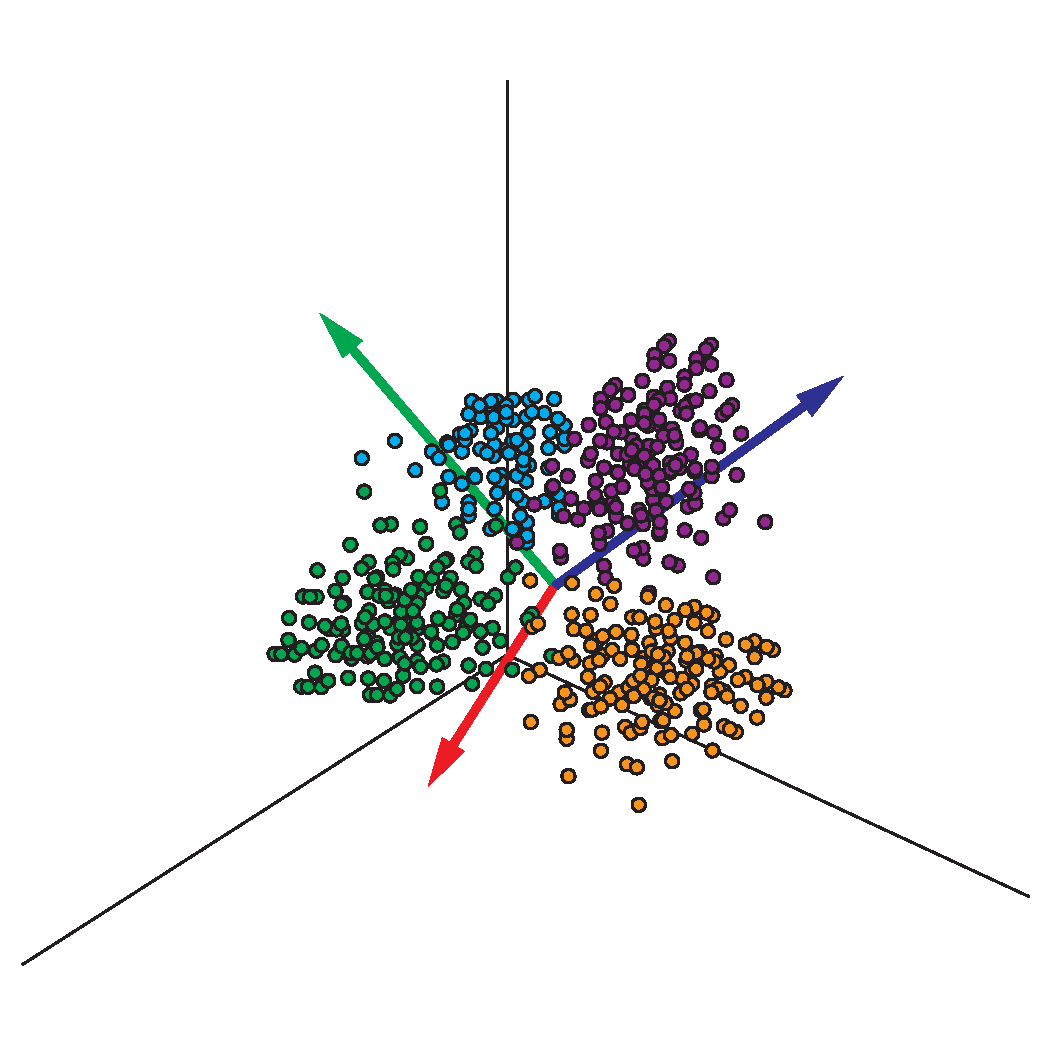
\includegraphics[valign=t,frame,scale=0.4]
{diagrams/pca-3d.pdf}%
\label{fig:DimRed3D}%
}
\hfill         % fills up the space between the two graphics
\subfloat[%
Scatter plot after PCA reduced from 3 dimensions to 2 dimensions.] {%
\includegraphics[valign=t,frame,scale=0.4]
{diagrams/pca-2d.pdf}%
\label{fig:DimRed2D}%
}

\caption[Dimensionality Reduction with PCA]
{Data visualisation before and after dimensionality reduction with the PCA
method.
\imgcredit{Both images created by Ožbej Golob.}
}
\label{fig:DimRed}
\end{figure}


\subsection{Principal Component Analysis (PCA)}

Principal Component Analysis (PCA) is a linear projection. PCA uses linear
algebra to identify the underlying dimensions or factors in the data and
project the data onto a lower-dimensional space.

The main goal of PCA is to identify patterns in data, which are often
hidden or difficult to detect. This is done by analyzing the covariance
matrix of the original dataset, which describes the relationship between
the different variables. By calculating the eigenvectors and eigenvalues
of the covariance matrix, PCA identifies the directions in which the data
varies the most, or the principal components. 

The principal components are ordered by the amount of variance they
explain in the original data. The first principal component explains the
largest amount of variance, followed by the second principal component,
and so on. By keeping only the principal components that explain the
majority of the variance in the data, the dimensionality of the dataset
can be reduced, while still retaining the most important information
\parencite{abdi2010principal}.


\subsection{Multi-Dimensional Scaling (MDS)}

Multi-Dimensional Scaling (MDS) is a non-linear projection. MDS is used to
visualize the similarity or dissimilarity between different objects or
observations. The technique transforms a set of high-dimensional data into
a lower-dimensional space, usually two or three dimensions, while
preserving the relationships between the data points.

MDS works by first calculating the pairwise distances or dissimilarities
between all the objects in the dataset. These distances could be based on
any metric, such as Euclidean distance, correlation distance, or other
similarity measures. Once the distance matrix is constructed, MDS tries to
find a configuration of points in a lower-dimensional space that best
reproduces the distances or dissimilarities between the original objects.
This is done by minimizing a cost function, such as stress or error, which
measures the discrepancy between the original pairwise distances and the
distances between the projected points.

MDS can be classified into two main types: metric and non-metric. In
metric MDS, the pairwise distances between the objects are preserved
exactly, while in non-metric MDS, only the rank order of the distances is
preserved. Non-metric MDS is often used when the underlying distance
metric is unknown or not easily quantifiable \parencite{morrison2003fast}.


\subsection{t-Distributed Stochastic Neighbor Embedding (t-SNE)}

t-Distributed Stochastic Neighbor Embedding (t-SNE) is a non-linear
projection. t-SNE uses a probabilistic model to preserve the local
structure of the data in the high-dimensional space and project the data
onto a lower-dimensional space, , usually two or three dimensions.

The t-SNE algorithm works by first calculating the pairwise similarities
between all the data points in the high-dimensional space. This is
typically done using a Gaussian kernel, which measures the similarity
between two points as a function of their Euclidean distance. The
similarities are then used to construct a probability distribution for
each point that defines the likelihood of finding other points nearby.

In the low-dimensional space, t-SNE tries to find a configuration of
points that preserves the pairwise similarities between the
high-dimensional data points as closely as possible. The algorithm does
this by minimizing a cost function that measures the divergence between
the probability distributions in the high-dimensional and low-dimensional
spaces. The optimization is performed using gradient descent, which
iteratively updates the position of each point in the low-dimensional
space until the cost function is minimized.

One of the key features of t-SNE is that it uses a Student's
t-distribution to model the probability distribution in the
low-dimensional space. This allows t-SNE to emphasize the differences
between nearby data points and de-emphasize the differences between
distant data points, which helps to prevent crowding and distortion in the
final visualization \parencite{van2008visualizing, wattenberg2016how}.


\subsection{Uniform Manifold Approximation and Projection (UMAP)}

Uniform Manifold Approximation and Projection (UMAP) is a non-linear
dimension reduction algorithm based on manifold learning techniques and
ideas from topological data analysis. UMAP is based on three assumptions
about the data: (i) The data has a uniform distribution of a Riemannian
manifold, (ii) The Riemannian metric is locally constant, and (iii) The
manifold is locally connected. UMAP uses these assumptions to model the
manifold with a fuzzy topological structure. The embedding is determined
by searching for a low-dimensional projection of the data that is the
closest equivalent to the fuzzy topological structure.

UMAP works by creating a low-dimensional representation of the data while
preserving the global structure of the data. This is achieved by modeling
the data as a high-dimensional manifold, which is a mathematical object
that represents the underlying structure of the data. UMAP then finds a
low-dimensional embedding of the manifold that preserves the local
structure of the data.

The UMAP algorithm consists of several steps. First, a nearest-neighbor
graph is constructed by connecting each data point to its nearest
neighbors. This graph is then used to create a fuzzy simplicial set, which
is a mathematical object that captures the local structure of the data.
The fuzzy simplicial set is then transformed into a low-dimensional
representation using a stochastic gradient descent algorithm.

UMAP has several advantages over other dimensionality reduction
techniques. For example, UMAP is able to preserve both the global and
local structure of the data, which means that it can be used for both
exploratory data analysis and machine learning tasks
\parencite{mcinnes2018umap}.


\subsection{Comparison of Similarity Mapping Techniques}

The following section is meant to illustrate how above mentioned
similarity mapping techniques work in practice on two well-known datasets.
All graphics in the following section are generated using Python with the
help of the following libraries: [TODO add libraries and cite them].

The \emph{Iris dataset}~\parencite{fisher1936use} is arguably the best
known dataset in the pattern recognition literature. The dataset contains
150 instances belonging to 3 classes of Iris flower species (each class
has 50 instances). Each instance has the following attributes: sepal
length in cm, sepal width in cm, petal length in cm, and petal width in
cm. Each instance belongs into one of 3 classes: Iris Setosa, Iris
Versicolour, or Iris Virginica. Iris Setosa is linearly separable from the
other 2, and the latter are not linearly separable from each other.
Figure~\ref{fig:IrisDataset} shows comparison of similarity mapping
techniques on the Iris dataset. It is visible that all techniques separate
Iris Setoca class from the other two, while the other two can not be
clearly separated from each other. t-SNE and UMAP techniques generate
dense clusters while PCA and MDS clusters are more sparse.

The \emph{Palmer Penguins dataset}~\parencite{gorman2014ecological,
horst2020penguins} contains 342 instances belonging to 3 classes of
penguin species from Antarctica (from Torgersen, Biscoe, and Dream
islands). Each instance has the following attributes: island, bill length
in mm, bill depth in mm, flipper length in mm, body mass in g, sex, and
year. Each instance belongs into one of 3 classes: Adelie, Gentoo, or
Chinstrap. Figure~\ref{fig:PenguinDataset} shows comparison of similarity
mapping techniques on the Palmer Penguins dataset. It is visible that all
techniques separate Gentoo class from the other two, while the other
two can not be clearly separated from each other. t-SNE and UMAP
techniques generate dense clusters while PCA and MDS clusters are more
sparse.

\begin{figure}[tp]
\centering
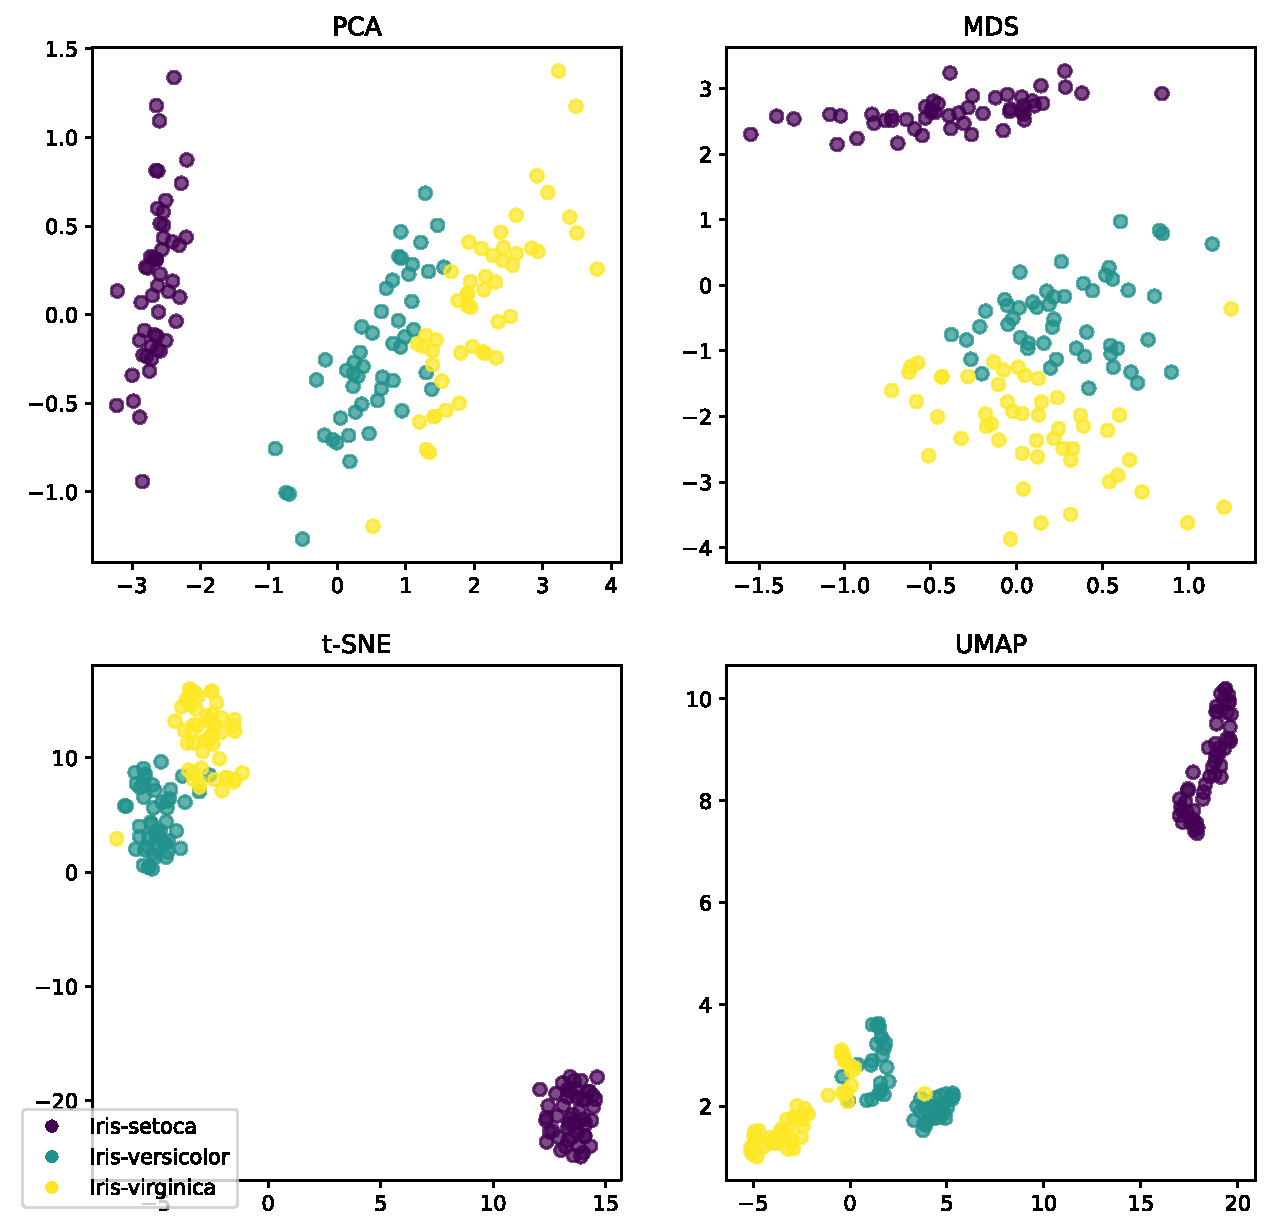
\includegraphics[frame,keepaspectratio,width=\linewidth,height=\halfh]
{diagrams/iris.pdf}

\caption[Similarity Mapping on Iris dataset]
{
  Comparison of similarity mapping techniques on the Iris dataset.
\imgcredit{Drawn by Ožbej Golob using Python.}
}
\label{fig:IrisDataset}
\end{figure}


\begin{figure}[tp]
\centering
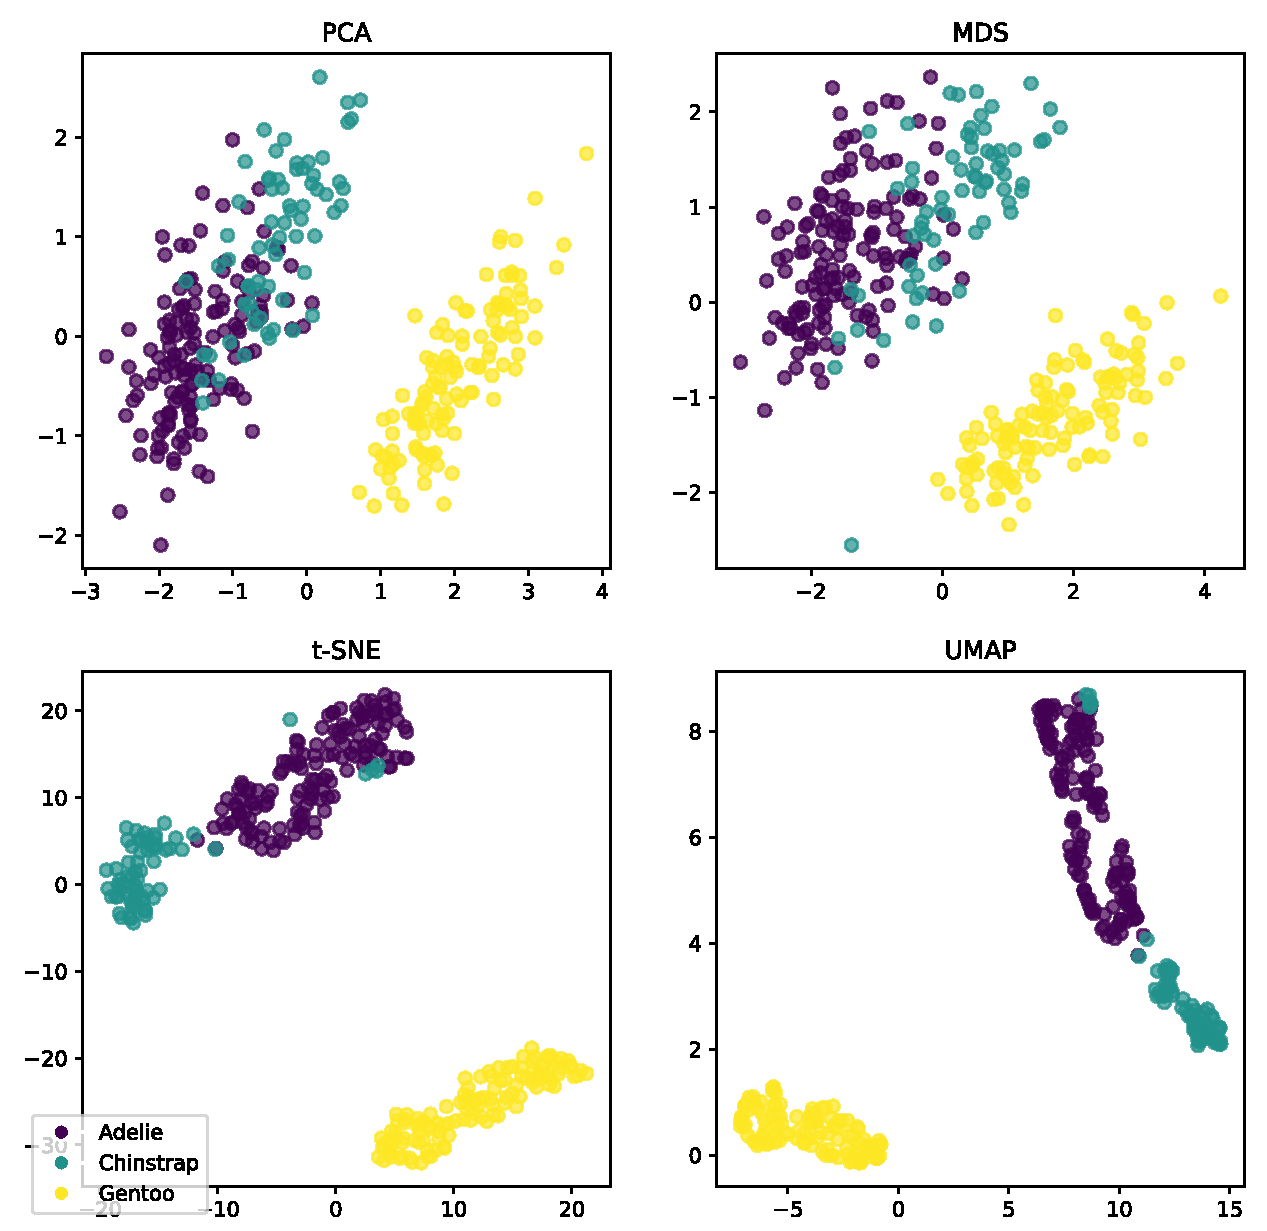
\includegraphics[frame,keepaspectratio,width=\linewidth,height=\halfh]
{diagrams/penguins.pdf}

\caption[Similarity Mapping on Palmer Penguins dataset]
{
  Comparison of similarity mapping techniques on the Palmer Penguins
  dataset.
\imgcredit{Drawn by Ožbej Golob using Python.}
}
\label{fig:PenguinDataset}
\end{figure}


\section{Parallel Coordinates}

Parallel coordinates are a type of chart that is used to visualize
multi-dimensional data. In this type of chart, each data point is
represented by a vertical line that extends across multiple axes. The axes
are typically arranged in parallel. Each axis represents a different
variable, and the position of a point on that axis indicates the value of
that variable for the data point. This allows multiple variables to be
compared and analyzed simultaneously \parencite{inselberg1990parallel}.
Figure~\ref{fig:ParallelCoordinatesDiagram} shows an example of a parallel
coordinates plot displaying data points with multiple dimensions.

\begin{figure}[tp]
\centering
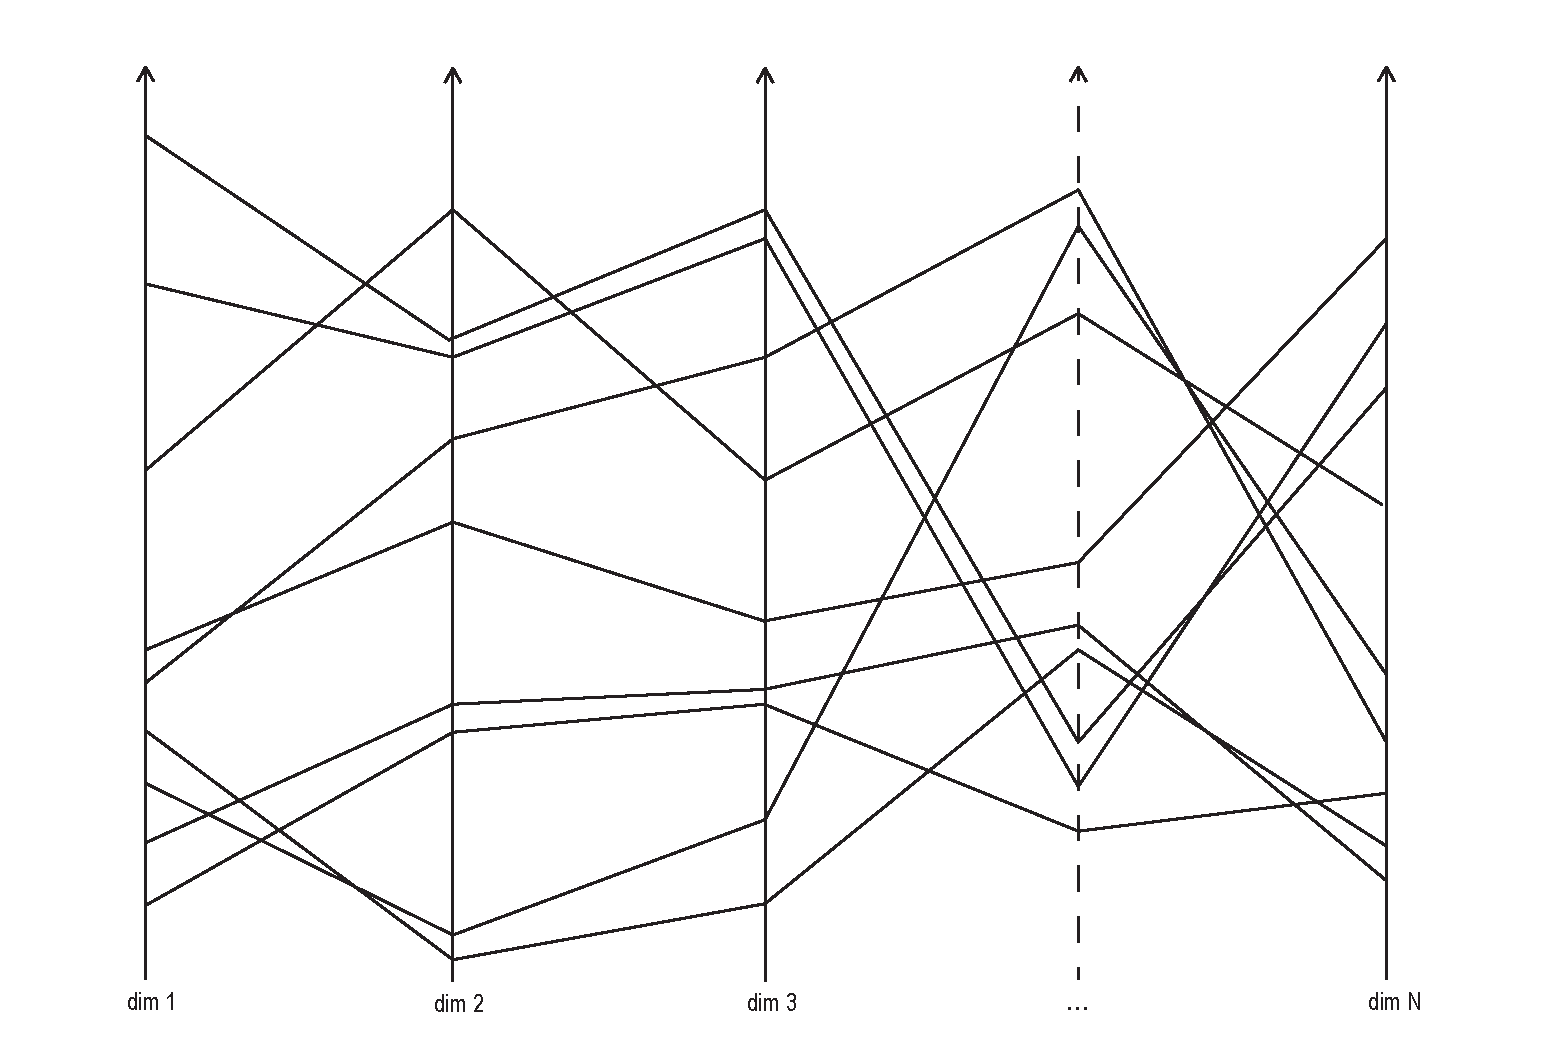
\includegraphics[frame,keepaspectratio,width=\linewidth,height=\halfh]
{diagrams/parallel-coordinates.pdf}

\caption[Parallel Coordinates]
{
A parallel coordinates plot displaying data points with multiple dimensions.
\imgcredit{Drawn by Ožbej Golob using Adobe Illustrator.}
}
\label{fig:ParallelCoordinatesDiagram}
\end{figure}






\section{Brushing and Linking}

Brushing and linking are techniques used in multidimensional visual
analysis to allow the user to interact with a visualization and
explore data in greater depth.

Brushing refers to the process of selecting data points or regions in one
visualization and highlighting those data points in other visualizations.
This allows the user to see how the data points or regions of interest are
related to other variables in the dataset.
Figure~\ref{fig:BrushingDiagram} shows an example of brushing. The user
selected a single data point which is now highlighted in all views with
red color.

Linking refers to the process of synchronizing the views of multiple
visualizations, such that a change made to one visualization is
reflected in the other visualizations. This allows the user to explore
the data from different perspectives and understand how different
variables are related to one another.

Both brushing and linking are useful for helping users to identify
patterns and relationships in the data and for facilitating the
process of data exploration and analysis.

\begin{figure}[tp]
\centering
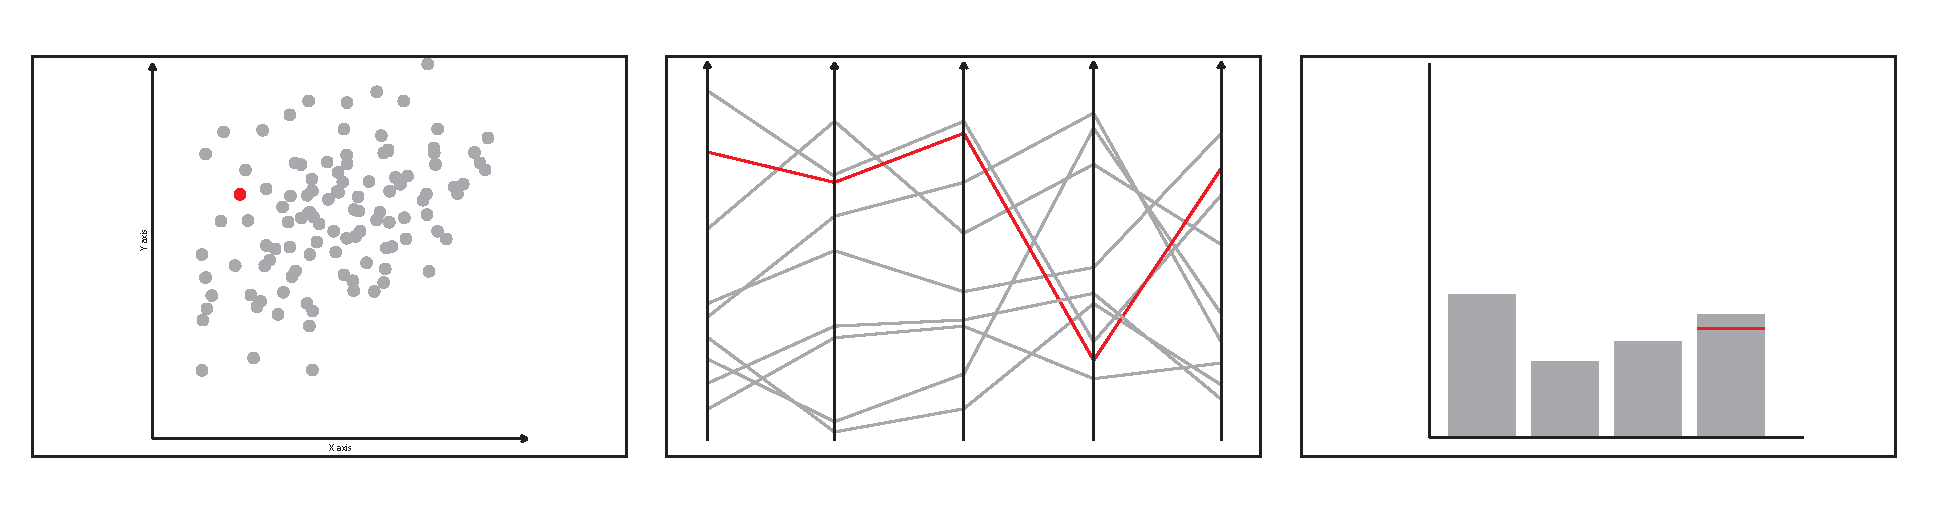
\includegraphics[frame,keepaspectratio,width=\linewidth,height=\halfh]
{diagrams/brushing.pdf}

\caption[Brushing]
{ An example of brushing. The user selected a single data point which
is now highlighted in all views with red color.
\imgcredit{Drawn by Ožbej Golob using Adobe Illustrator.}
}
\label{fig:BrushingDiagram}
\end{figure}




\section{Grouping and Labelling}

Grouping and labeling data is a fundamental step in the Machine Learning
(ML) process. Grouping refers to the process of identifying and separating
similar data points, while labeling refers to the process of providing
relevant information about the data. Grouping and labelling data helps to
organize and structure the data, making it easier to understand and work
with. It allows for more accurate and meaningful analysis of the data, as
similar data points can be grouped together and analyzed in relation to
one another. It also allows the ML model to understand the context of the
data and make more accurate predictions, and enables the interpretability
of the model, by providing meaningful information about the data and how
it is being used.

\subsection{Manual Grouping}

Manual grouping and labeling refers to the process of organizing and
providing relevant information about data manually, typically done by a
human. The process of manual grouping and labeling can be time-consuming
and labor-intensive.




\subsection{Automated Clustering}

Cluster analysis is a type of mathematical methods used to identify which
objects in a given data set are similar. It is a commonly used method for
exploratory data analysis, and is often used as a way to gain insight into
the underlying structure of the data. Cluster analysis methods sort
objects described as data. Objects with similar descriptions are grouped
into the same cluster. This allows analysts to identify common patterns
and trends within the data, and to gain a better understanding of the
relationships between the objects in the data set
\parencite{romesburg1984cluster}.



